\chapter{Generación de lenguaje natural}
\label{cap:nlg_intro}
La generación de lenguaje natural (NLG) es un una rama de la lingüística computacional y la inteligencia artificial encargada de estudiar la construcción de sistemas computacionales capaces de producir texto en castellano o cualquier otra lengua humana a partir de algún tipo de representación no-lingüística de la información a comunicar. Estos sistemas combinan conocimientos tanto del lenguaje en cuestión como del dominio de aplicación para producir automáticamente documentos, reportes, mensajes o cualquier otro tipo de textos.

Dentro de la comunidad de investigación y desarrollo de la NLG hay un cierto consenso sobre la funcionalidad lingüística general de un sistema de NLG.
En este trabajo se optó por seguir la metodología más comúnmente aceptada, propuesta por Reiter y Dale~\cite{reiter_dale}.
A continuación se describirán brevemente los aspectos más importantes de esta metodología y en capítulos posteriores se desarrollarán más en profundidad los puntos más relevantes para nuestro trabajo.

\section{Análisis de requerimientos}
El primer paso en la construcción de cualquier sistema de software, incluyendo los sistemas de generación de lenguaje natural, será el de realizar un análisis de requerimientos y a partir de ahí generar una especificación inicial del sistema. 

Para el análisis de requerimientos, Reiter y Dale proponen realizar un corpus de textos de ejemplo y a partir de ellos obtener una especificación para el sistema a desarrollar. Estos ejemplos estarán compuestos por una colección de datos de entrada del sistema con sus respectivas salidas (texto en lenguaje natural). Estos deberán estar redactados por un humano experto y deberían caracterizar lo mejor posible todas las salidas posibles que se espera que el sistema genere.

En el capítulo~\ref{cap:corpus} se profundizará más sobre este tema, describiendo y analizando el \emph{corpus de descripciones} utilizado para este trabajo.

\section{Tareas de la generación de lenguaje natural}
\label{sec:tareas_nlg}

La clasificación de Reiter y Dale distingue las siguientes siete tareas que deben ser realizadas a lo largo de todo el proceso de generación de lenguaje natural: 

\bigskip
\noindent
\textbf{Determinación del contenido:} es el proceso de determinar qué información debe ser comunicada en el texto final; será el encargado de que el mismo contenga toda la información requerida por el usuario. Generalmente involucra una o más tareas de selección, resumen y razonamiento con los datos de entrada.

\bigskip
\noindent
\textbf{Estructuración del documento:} es el proceso de imponer un orden y estructura sobre los textos a generar a fin de que la información del documento final se encuentre estructurada de forma entendible y fácil de leer.

\bigskip
\noindent
\textbf{Lexicalización:} es el proceso de decidir qué palabras y frases especificas usar para expresar los distintos conceptos y relaciones del dominio. En esta etapa se deberá establecer cómo se expresa un significado conceptual concreto, descrito en términos de un modelo del dominio, usando elementos léxicos (sustantivos, verbos, adjetivos, etc).

\bigskip
\noindent
\textbf{Generación de expresiones de referencia:} es la tarea de elegir qué expresiones usar para identificar entidades del dominio de aplicación. Podríamos querer referirnos a una determinada entidad de distintas formas. Por ejemplo: podríamos querer referirnos al mes en curso como ``febrero'', ``este mes'', ``éste'', etc.

\bigskip
\noindent
\textbf{Agregación:} se encarga de combinar dos o más elementos informativos con el fin de conseguir un texto más fluido y legible. La agregación decide qué elementos se pueden agrupar para generar oraciones más complejas sin modificar el significado de las mismas. Por ejemplo, dos frases de una descripción para una clase de prueba de un \textit{scheduler} se podrían expresar como:
\emph{``El proceso a borrar se encuentra en la tabla de procesos. El estado del proceso a borrar es waiting.''} o \emph{``El proceso a borrar se encuentra en la tabla de procesos y el estado del mismo es waiting.''}

\bigskip
\noindent
\textbf{Realización lingüística:} es el proceso de aplicar reglas gramaticales (a estructuras generadas por las etapas anteriores) con el fin de producir un texto que sea sintáctica, morfológica y ortográficamente correcto.

\bigskip
\noindent
\textbf{Realización de la estructura:} esta tarea se encarga de convertir estructuras abstractas como párrafos y secciones (generadas por etapas anteriores) en texto comprensible por el componente de presentación del documento. Por ejemplo, la salida del sistema de NLG podría ser código LaTeX para luego ser post-procesado, en este caso sería esta etapa la encargada de agregar delimitadores y comandos de LaTeX para generar el documento. 

\section{Arquitectura para \textit{NLG}}
Existen muchas maneras de construir un sistema que realice las tareas antes mencionadas. Una forma podría ser construir un único módulo encargado de llevar a cabo todas las tareas en simultaneo. En el otro extremo, podríamos tener un módulo separado para cada tarea y conectarlos mediante un \emph{pipeline}. En este caso, el sistema primero se encargaría de la determinación de contenido, luego la estructuración del documento, y así sucesivamente. La desventaja de este último modelo es que asume que las tareas deben ser realizadas en un único orden y que las funcionalidades de las mismas no se solapan.

En este trabajo se utilizará la arquitectura, más comúnmente utilizada para sistemas de NLG, introducida también por Reiter y Dale~\cite{reiter_dale}. Estos proponen una arquitectura que se encuentra en el medio de los dos extremos antes mencionados, donde las tareas antes mencionadas (sección \ref{sec:tareas_nlg}) son agruparas y llevadas a cabo en conjunto en tres grandes etapas: \emph{document planning}, \emph{microplanning} y \emph{surface realization}. La arquitectura propuesta consiste en tres módulos conectados mediante un \emph{pipeline}, donde cada uno de estos se encargará de una de las etapas recién mencionadas. En la figura \ref{fig:png_arquitectura} podemos observar los tres módulos que componen este \emph{pipeline}; a continuación se detallarán brevemente las tareas a realizar en cada una de estos.

\begin{figure}[h]
  	\centering
	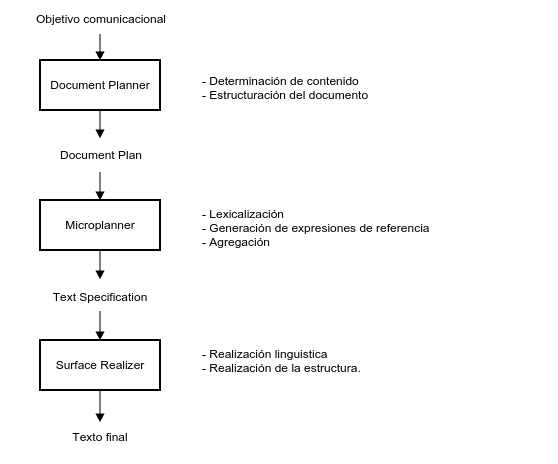
\includegraphics[scale=0.6]{img/arquitectura.png}
	\caption{Arquitectura típica de un sistema NLG}
  	\label{fig:png_arquitectura}
\end{figure}

El primer módulo de nuestro sistema será el \emph{document planner}, encargado de realizar las tareas de determinación de contenido y estructuración del documento. Veremos en el capítulo~\ref{cap:document_planning} que estas tareas se encuentran sumamente relacionadas y son realizadas en simultaneo. La salida de esta etapa y entrada del \emph{microplanner} será un \emph{document plan}, éste será una abstracción del documento final que contendrá los elementos informativos que se desea comunicar.

El segundo módulo será el encargado de realizar las tareas de lexicalización, generación de expresiones de referencia y agregación. La función del mismo será la de trabajar el \textit{document plan} generando una especificación más refinada del texto final. El \emph{microplanner} será el responsable de transformar los elementos informativos incluidos en el \textit{document plan} en una especificación más concreta de una oración. En el capítulo~\ref{cap:microplanning} se desarrollará más en profundidad el funcionamiento del \textit{microplanner}.

Finalmente el \emph{surface realizer} tomará como entrada la especificación de texto generada por la etapa anterior y será el encargado de producir el texto final. Este módulo deberá llevar a cabo las tareas de realización lingüística y de estructural antes mencionadas.

\section{Resumen del capítulo}
En este capítulo se presentó la metodología propuesta por Reiter y Dale, viendo las tareas básicas que un sistema de generación de lenguaje natural debe llevar a cabo. 

Como se mencionó anteriormente, si bien se seguirá la metodología mencionada, en este trabajo se desarrollarán las particularidades necesarias para aplicar la misma a nuestro problema, la generación de descripciones en lenguaje natural para las clases de prueba del TTF. En el capítulo \ref{cap:corpus}, daremos el primer paso necesario para la construcción de este sistema realizando un análisis detallado del corpus de descripciones a fin de obtener los requerimientos necesarios. En el capítulo \ref{cap:document_planning} estudiaremos más en detalle la etapa de \textit{document planning}, donde veremos las tareas de determinación de contenido y estructuración del documento, dependientes del dominio de aplicación con el que se ha trabajado (las clases de prueba del TTF). En el capítulo \ref{cap:microplanning} se desarrollará la etapa de \textit{microplanning} de nuestro sistema, donde veremos, entre otras cosas, la tarea de lexicalización resultado del conjunto de reglas recolectadas para este trabajo; las cuales se introducirán en el capítulo \ref{cap:corpus}. Finalmente, en el capítulo \ref{cap:realization} se desarrollará un pequeño realizador lingüístico en español, necesario para la última la etapa de \textit{surface realization} de la arquitectura presentada.

